\section{Detailed control design for agreed plant section}
\label{sec:subsec}

\subsection{Description of sub-section}
The agreed subsection begins with a gaseous \ch{H2} stream and liquid methanol and o-nitrotoluene stream. The \ch{H2} stream is driven through a fan and preheated by an electric heater (H201) before being fed to a trickle bed reactor (R201). The liquid stream is pumped through P201 and also preheated by an electric heater (H202) and then enters R201. The reactor has a gaseous effluent which is split into a recycle and purge stream. The liquid effluent enters a packed distillation column (S201), where methanol is separated from the heavier organics. The methanol-rich vapour from the column is partially condensed and split into a gaseous and liquid product in a reflux drum (S204), while the bottoms stream containing valuable o-toluidine product is sent to downstream purification units.

\subsection{Degree of freedom analysis}
To understand the number of variables that can be simultaneously manipulated to maintain stable operation, a degree of freedom analysis was carried out. A thorough analysis involves subtracting the total number of variables from the total number of equations in a dynamic model of each process unit, however creating a dynamic model is often impractical and error-prone for complex plants with specialised units. Instead, the simpler and straightforward method presented by \textcite{} is used, and the results are presented in Table XX.

\subsection{Key control loops}
\Cref{tab:controls} shows a summary of the control loops in the plant sub-section. A total of 14 variables were controlled using feedback, feedforward, cascade, ratio and inferential control in order to ensure stable operation of the units in the sub-section.

\begin{table}[h]
\centering
    \caption{Summary of control loops}
    \label{tab:controls}\footnotesize
\adjustbox{max width=\textwidth}{
\begin{tabular}{p{3cm}|p{3cm}|p{4cm}|p{5cm}|p{6cm}}
\toprule
\textbf{Unit}                               & \textbf{Controlled Variable}                & \textbf{Manipulated Variable}                           & \textbf{Sensor/Actuator}                                                   & \textbf{Control Strategy}                                                                                                            \\ \midrule
\multirow{7}{*}{Reactor (R201)}             & Temperature of reactor                      & Cooling water flowrate in reactor jacket                & Temperature sensor (TT-201) / Flow control valve (FCV-201)                 & Feedforward control mitigates temperature disturbances and cascade   control counters flow disturbances in cooling water.            \\
                                            & Pressure of reactor                         & Pressure of the fresh hydrogen                          & Pressure sensor (PT-201) / Pressure control valve (PCV-202)                & Feedforward control mitigates disturbances in upstream fresh H­2 pressure and recycle H2 pressure.                                   \\
                                            & Ratio of reactants                          & Flowrate of fresh methanol                              & Flow sensors (FT-202, FT-203) / Pump speed (P201)                          & Ratio control ensures the H2 and liquid feed enter the reactor in fixed proportions.                                                 \\
                                            & Composition of gas feed to reactor          & Flowrate of purge                                       & Composition analyser (AT-203) / Flow control valve (FCV-203)               & Cascade control allows composition to be manipulated using the purge   flowrate which is a slave control to smooth any disturbances. \\
                                            & Level                                       & Flowrate of reactor outlet                              & Level transmitter (LT-208) / Flow control valve (FCV-203)                  & Level control is cascaded to flow control.                                                                                           \\
                                                                                        & Hydrogen flowrate                                     & Fan motor speed                              & Flow transmitter (LT-208) / Fan motor (F201)                  & Feedback control to maintain stable unit operation.                                                                                           \\
                                                                   
                                                                                        \midrule
Electric Heaters (H201 / H202)              & Temperature of outlet streams               & Electrical input to heater                              & Temperature sensor (TT-202, TT-212) / Heaters (H201, H202)                 & Feedback control maintains stable unit operation.                                                                                    \\ \midrule
\multirow{3}{*}{Distillation Column (S203)} & Bottoms composition                         & Steam flowrate to reboiler (reboiler duty)              & Composition analyser (AT-205) / Flow control valve (FCV-207)               & Composition control is cascaded to inferential temperature control to   increase the responsiveness of control.                      \\
                                            & Pressure of column        & Gas   flowrate vented from reflux drum & Pressure   sensor (PT-206) / Flow control valve (FCV-205) & Feedback   control maintains stable unit operation.                                                                \\
                                            &                                             &                                                         &                                                                            &                                                                                                                                      \\
                                            & Feed   pressure                             & Valve position                                          & Pressure sensor (PT-208) / Pressure control valve (PCV-201)                & Feedback control minimises pressure disturbances to the column.                                                                      \\ \midrule
Reboiler (H204)                             & Level in the reboiler                       & Flowrate of bottoms product                             & Level sensor (LT-202) / Flow control valve (FCV-208)                       & Feedback control maintains stable unit operation.                                                                                    \\ \midrule
Reflux Drum (S204)        & Level in   the reflux drum & Flowrate   of tops product            & Level   sensor (LT-203) / Flow control valve (FCV-206)   & Feedback   control is coupled with feedforward control to smooth disturbances in feed flowrate.                   \\
                                            &                                             &                                                         &                                                                            &                                                                                                                                      \\ \midrule
Partial Condenser (H203)                    & Condenser duty                              & Temperature of cooling water                            & Temperature sensor (TT-208) / Flow control valve (FCV-204)                 & Temperature control is cascaded to flow control to smooth upstream   disturbances from the cooling water.                            \\ \bottomrule
\end{tabular}}
\end{table}


\subsubsection{Reactor R201 temperature control} %R201-TC
Robust control of the reactor temperature is essential to minimise the risk of thermal runaway of the highly exothermic hydrogenation reaction. The temperature of R201 is controlled using the cooling water flowrate throuch the cooling jacket. A control system encompassing a feedback control loop, two feedforward controllers and cascade control was designed. The master temperature controller infers a set point to the slave flow controller which acts on the flow control valve installed on the cooling water inlet stream. Three major disturbances where identified: the cooling water pressure, the cooling water temperature and the temperature of the gas feed to the reactor. For the later two, additional feedforward control was implemented in order for the system to adjust before it is reached by the disturbances. The temperature of the gas feed was deemed a more major disturbance than the temperature of the liquid feed since they are fed to the reactor in a 4 to 1 ratio. The disturbances in the cooling water feed pressure, originating from the high demand for cooling water on the plant, are accounted for by the cascade control loop.

\begin{figure}[h]
    \centering
    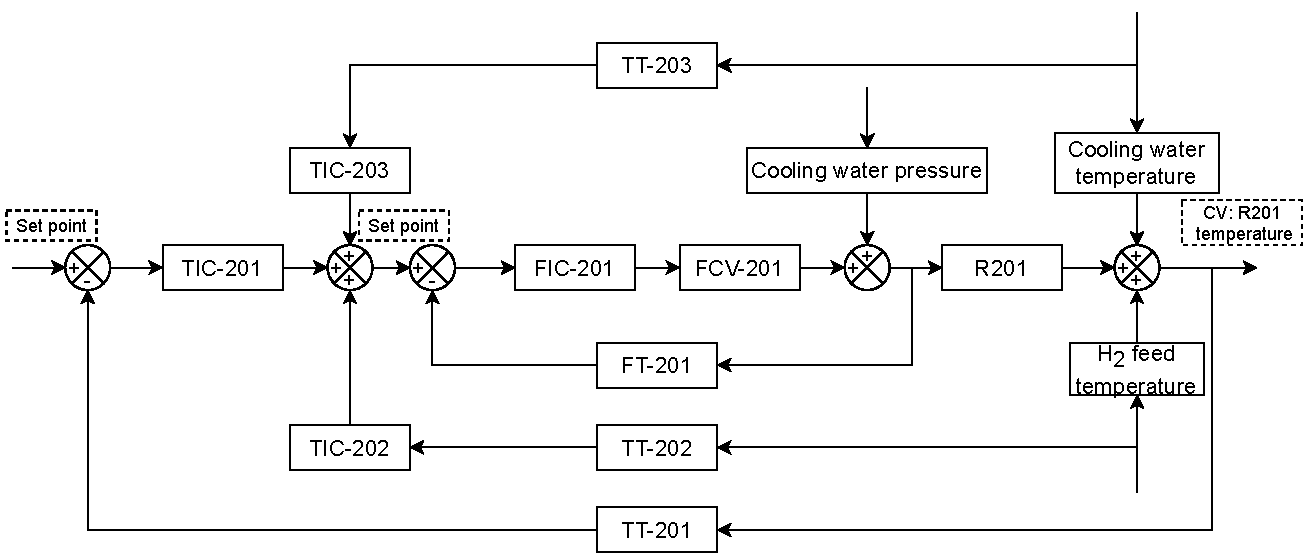
\includegraphics[width=0.8\linewidth]{chapters/4-operation-control/4-Figures/R201-TC.pdf}
    \caption{Temperature control loop for reactor R201}
    \label{fig:R201-TC}
\end{figure}

\subsubsection{Reactor R201 pressure control} %R201-PC
The ONT reduction reactor is operated under pressure at 5 atm. To maintain this optimum operating condition and most importantly reduce the risk of overpressure and explosion, the pressure within the reactor is closely monitored and controlled. The manipulated variable is the pressure of the  

\begin{figure}[h]
    \centering
    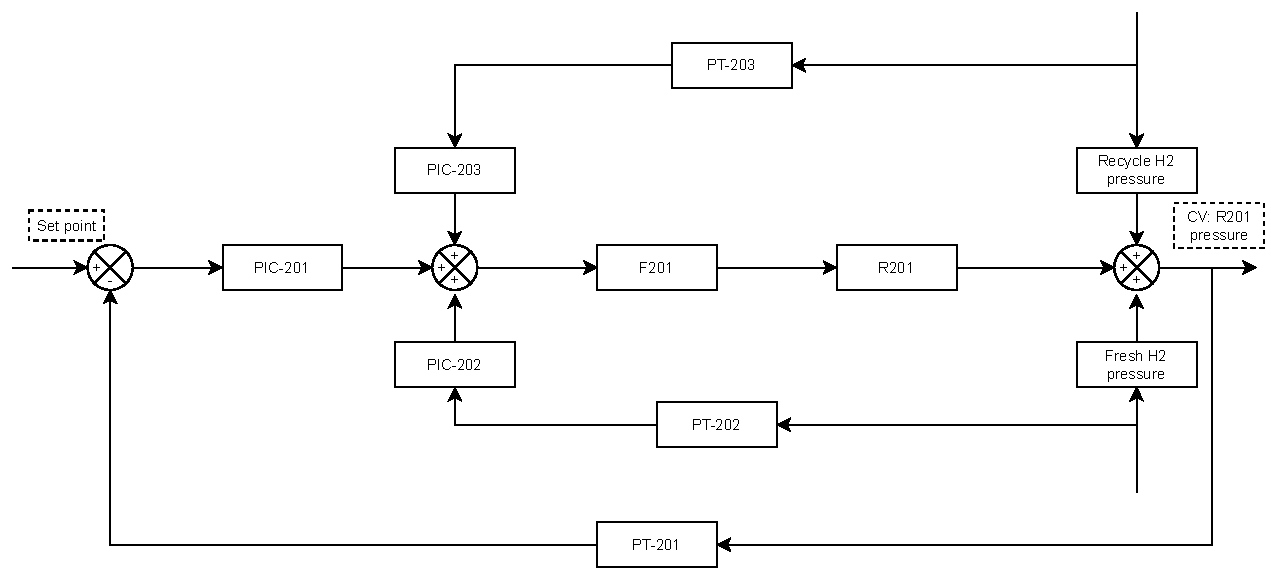
\includegraphics[width=0.8\linewidth]{chapters/4-operation-control/4-Figures/R201-PC.pdf}
    \caption{Pressure control loop for reactor R201}
    \label{fig:R201-PC}
\end{figure}

\subsubsection{Ratio control of reactants} %R201-CC
\begin{figure}[h]
    \centering
    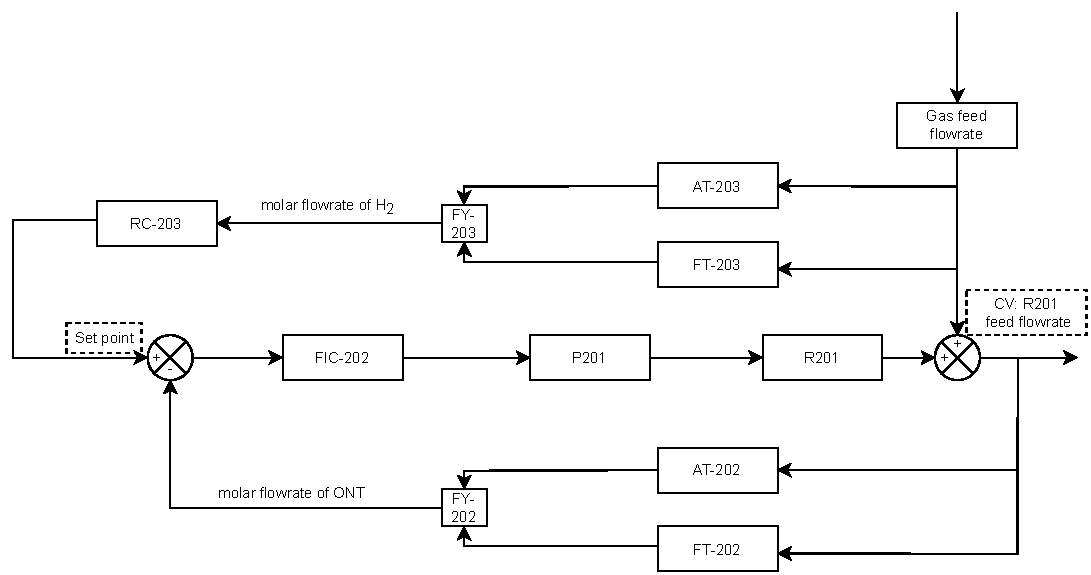
\includegraphics[width=0.8\linewidth]{chapters/4-operation-control/4-Figures/R201-FC.pdf}
    \caption{}
    \label{fig:R201-FC}
\end{figure} 

\subsubsection{Hydrogen recycle control}%V202-CC
\begin{figure}[h]
    \centering
    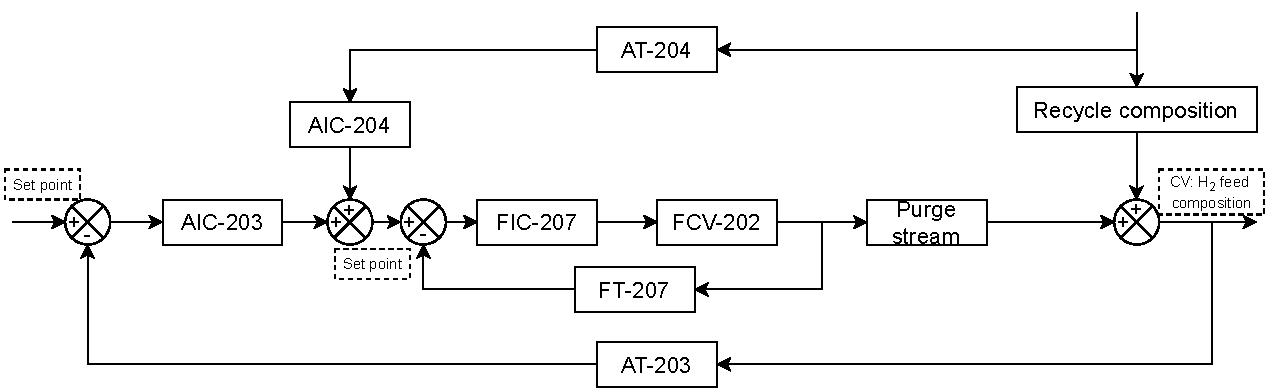
\includegraphics[width=0.8\linewidth]{chapters/4-operation-control/4-Figures/V202-CC.pdf}
    \caption{}
    \label{fig:V202-CC}
\end{figure}

\subsubsection{Reactor R201 level control} % R201-LC


\subsubsection{Hydrogen feed flowrate} %R201-HFC
%no graph








\subsubsection{Reactor feed temperature control}%H201 and H202-TC 
%no graph

\subsubsection{Bottom stream composition control} %S201-CC
A composition control loop in the distillation column is also necessary to ensure a high recovery of o-toluidine. Since o-toluidine is found in the bottoms stream, reboiler duty was chosen as the manipulated variable in order to reduce the lag time of the controller. A composition analyser (AT-205) measures the concentration of o-toluidine in the bottoms stream and a composition controller (AIC-205) controls the reboiler duty by manipulating a flow control valve (FCV-207) on the saturated steam. 

A composition analyser was chosen to allow direct online measurements of the o-toluidine concentration, providing primary data to plant operators regarding this important performance indicator. However, composition analysers often have a slow dynamic response, leading to long measurement lags that result in a delay in the response of the control system. This sluggish behaviour would lead to the concentration of the bottoms fluctuating. To mitigate this, the temperature of the column is used as an inferential sensor to control the product composition, and is assigned as a slave controller under the master composition controller. Temperature sensors have quicker dynamic responses and can be correlated well to product composition. Controlling the temperature of the column is also crucial to a safe operation of the plant. Figure \ref{fig:S201-CC} shows the temperature controller (TIC-207) that receives its setpoint from the master composition controller (AIC-205), and outputs a signal to the flow control valve FCV-207.

\begin{figure}[h]
    \centering
    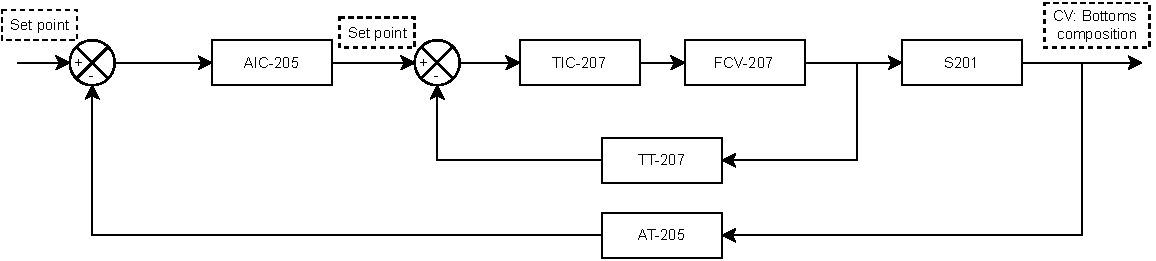
\includegraphics[width=0.8\linewidth]{chapters/4-operation-control/4-Figures/S201-CC.pdf}
    \caption{}
    \label{fig:S201-CC}
\end{figure}



\subsubsection{Distillation column S201 pressure control} %S201-PC
Pressure in distillation columns is regarded as one of the most important parameters to control well, as it not only affects the relative volatilities of the heavy and light keys, but also the shape of the vapour-liquid phase equilibrium curves which determine the compositions of the top and bottoms products of the distillation column. There are several options for for pressure control, such as controlling the vapour flow that is vented from the reflux drum, condenser duty, reboiler duty, recirculation of cooling fluid in the condenser or addition of inerts. Hence the choice of manipulated variable needs to be made carefully considering the relative direct impacts and time delays of each manipulated variable. Controlling the vapour flow that is vented from the reflux drum is the simplest control to implement and usually provides the fastest response as the amount of gas holdup in the column directly affects its pressure. In addition, the amount of vapours in the reflux drum S204 is much larger compared to the condensed liquid flow, so the direct impact of vapour flowrate on column pressure would be large. This avoids a situation where the flow control valve becomes saturated and unable to regulate pressure effectively. 

An optimal feedback control was designed with the vapour flowrate from the reflux drum as the manipulated variable. A pressure transmitter (PT-206) measures the pressure in the column, which is monitored by a pressure controller (PIC-206) that regulates a flow control valve (FCV-205) on the vent stream from the reflux (Figure \ref{fig:S203-PC}.

%no graph
%\begin{figure}[H]
 %   \centering
  %  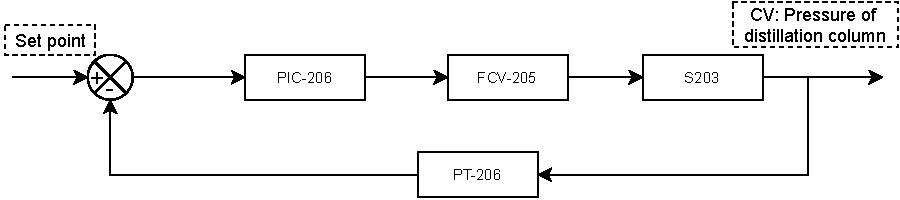
\includegraphics[width=\linewidth]{chapters/4-operation-control/4-Figures/S203-PC.pdf}
   % \caption{}
    %\label{fig:S203-PC}
%\end{figure}


\subsubsection{Control of pressure reduction valve V201} %V201-PC
To further ensure tight control of pressure in the column, a feedback control loop controls a pressure control valve on the feed to the column to minimise disturbances to the pressure of the feed to the column (see Figure \ref{fig:V201-PC}). %no graph

%\begin{figure}[H]
 %   \centering
  %  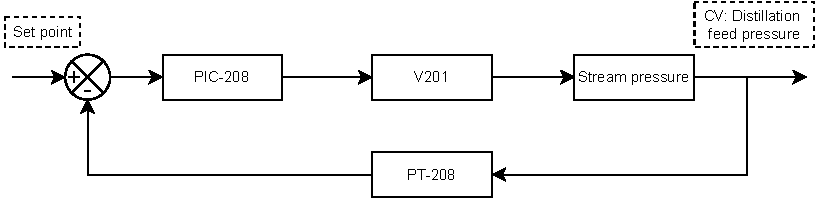
\includegraphics[width=\linewidth]{chapters/4-operation-control/4-Figures/V201-PC.pdf}
   % \caption{}
    %\label{fig:V201-PC}
%\end{figure}




%\subsubsection{Distillation column S201 level control}
%The liquid level at the bottom of the distillation column S201 is an important inventory to control to to prevent the reboiler from drying up and weeping to occur in the column. Since the reboiler duty is already being used in composition control, the most direct way of controlling the level is the bottoms flowrate out of the reboiler. Since the column and reboiler are connected, draining more liquid from the reboiler would draw more liquid from the column and vice versa. Due to the reboiler being able to store a certain amount of liquid inventory, a lag between the response of the actuator and the level is expected. While in most cases a simple feedback controller is sufficient (see Figure \ref{fig:S203-LC}, experimental data would confirm if more advanced systems are needed to compensate for a large time delay. 

%\begin{figure}[H]
   % \centering
   % 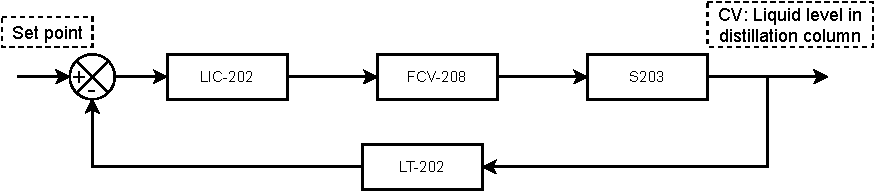
\includegraphics[width=\linewidth]{chapters/4-operation-control/4-Figures/S203-LC.pdf}
  %  \caption{}
  %  \label{fig:S203-LC}
%\end{figure}

\subsubsection{Reboiler H204 level control} %H204-LC
%no graph


\subsubsection{Reflux drum S204 level control}%S204-LC
Similar to the level control in the column, controlling the level of liquid in the reflux drum is required for stable operation of the column. Letting the drum run dry would lead to no reflux returning to the column, which would affect the separation efficiency of the light and heavy components. The manipulated variable for the liquid level was chosen to be the tops product flowrate, as it was desirable to maintain a constant reflux ratio to the column in order that the energy required to achieve the desired degree of separation would remain constant. A level transmitter (LT-203) sends a signal to the level controller (LIC-203) which controls a flow control valve (FCV-206) on the tops outlet stream, as shown on the P\&ID. 


\subsubsection{Heat duty of condenser H203 control}%H203-TC
The condenser in a distillation column provides cooling to condense the vapour exiting from the top of the column. It is usually desirable to operate the condenser at maximum duty, as reflux to the column has to be in a liquid state. Thus it is important to ensure that any disturbances to the cooling water flowrate and temperature are mitigated with a control loop. A cascade control was proposed, with the slower temperature loop as the master control and flowrate as the slave (see Figure \ref{fig:S203C-TC}). This way, any disturbances in the flow can be quickly rectified by the flow controller (FIC-208), while the temperature controller (TIC-208) gradually modifies the overall setpoint for the flow to account for disturbances in temperature.

\begin{figure}[h]
    \centering
    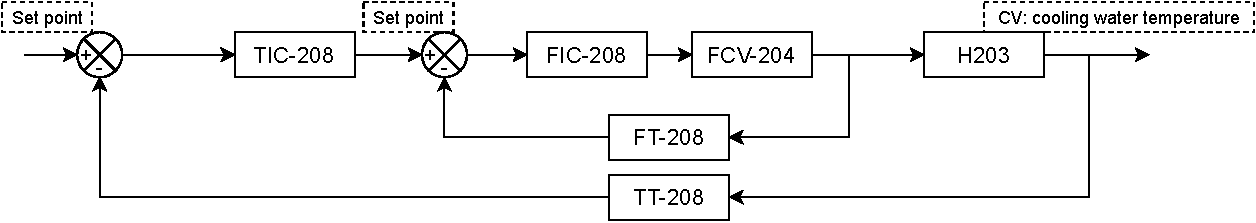
\includegraphics[width=0.8\linewidth]{chapters/4-operation-control/4-Figures/H203-TC.pdf}
    \caption{}
    \label{fig:S203C-TC}
\end{figure}



\subsection{Safety design}

\subsubsection{Alarms and emergency trips strategy}

\subsubsection{Alarms and safety interlocks design}